\section{Introducción}
%\flushleft\includegraphics[scale=0.75]{specification.pdf}
Este informe se propone abordar la resoulusión numérica de problemas de valores iniciales a través de los métodos Euler explícito, Euler implícito y Runge Jutta de orden 2. Se quiere resolver un sistema de suspensión vehicualer, el cual se modela como un sistema oscilatorio amortiguador expresado por una ecuación diferencial de segundo grado.
\section{Análisis}
Para empezar, realizamos un análisis del problema de forma física:
\begin{figure}[h] 
    \centering
    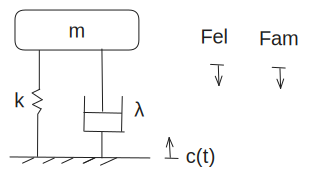
\includegraphics[width=0.5\textwidth]{imagenes/analisis.png}
    \caption{Análisis del caso de estudio}
    \label{fig:mi_figura}
\end{figure}

\begin{figure}[h] 
    \centering
    \includegraphics[width=0.5\textwidth]{imagenes/circuito.png}
    \caption{Circuito mecanico}
    \label{fig:mi_figura}
\end{figure}
El enunciado nos da una ecuación diferencial que es la siguiente:
\begin{align}
    y'' &= \frac{k}{m}(c - y) + \frac{\lambda}{m}(c' - y')
\end{align}
Esta representa la aceleración vertical de la carrocería. Es decir, oscilador amortiguado que responde a una excitación dada por la variable c.
\begin{itemize}
    \item \( k \) constante elástica del muelle [N/m]
    \item \( \lambda \) constante de amortiguación [Ns/m]
    \item \( c \) cota o elevación del terreno [m]
    \item \( y \) posición de la carrocería [m]
    \item \( c' \) y \( y' \) son derivadas de \( c \) e \( y \) con respecto al tiempo, es decir, velocidades verticales [m/s]
\end{itemize}
Entonces tenemos a \(c(t)\) y \(y(t)\) por hallar.
Como la solución general se solicita en el punto 1, desarrollaremos los métodos de forma genérica y luego se aplicará en el siguiente punto con lo solicitado.
Para ello debemos discretizar la EDO de segundo orden por los métodos propuestos.
Vamos a discretizar tres parámetros:
\subsection{Discretizar la EDO}
Como es una EDO de segundo orden se debe definir dos nuevas variables
\[
\begin{cases}
    y(t) \approx y(t_n) \approx u_n \\
    y'(t) \approx y'(t_n) \approx u'_n = v_n 
\end{cases}
\]
De esta forma pasamos de una EDO de segundo orden a una EDO lineal
\[
\begin{cases}
    u' = f_1(u,v,t) \\
    v' = f_2(u,v,t)
\end{cases}
\]